\section{Robustheit}\label{sec:robustheit}

Die Robustheit der Modelle wurde anhand zweier Kriterien bewertet: der Varianz der F1‑Scores über unterschiedliche Seeds und der Anzahl der Retries, die nötig waren, um eine formatkorrekte JSON‑Antwort von den \acp{LLM} in der Klassifizierungspipeline zu erhalten. Beide Größen geben Aufschluss darüber, wie stabil ein Modell im produktiven Einsatz ist.

Abbildung \ref{fig:results-evaluation-robustness-f1-std} zeigt die Standardabweichungen der F1‑Scores über fünf unabhängige Läufe mit unterschiedlichen Seeds. Die Mehrzahl der Modelle weisen Werte von deutlich unter $0{,}02$ auf. Sie liefern damit weitgehend gleiche Ergebnisse, unabhängig vom gewählten Seed, und gelten als stabil. Höhere Streuungen finden sich hingegen bei \texttt{Mistral Medium 3.1}, \texttt{Qwen2.5‑7B‑Instruct} und insbesondere \texttt{Mixtral‑8x7B‑Instruct‑v0.1}. Mit Standardabweichungen zwischen etwa $0{,}025$ und knapp über $0{,}04$ reagieren diese Modelle spürbar sensibler auf eine Änderung vom Seed. Ihre Leistung kann daher zwischen zwei Wiederholungen stärker schwanken.

Neben der Varianz des F1-Scores wurde die Zuverlässigkeit beim Einhalten des vorgegebenen Ausgabeformats betrachtet. Abbildung \ref{fig:results_evaluation_amount_of_retries} stellt die durchschnittliche Anzahl der Retries über alle Testfälle hinweg dar, die notwendig waren, bis eine gültige JSON-Antwort von den Modellen zurückgegeben wurde. Hier zeigen sich deutliche Unterschiede: Die meisten Modelle lieferten schon beim ersten Aufruf oder nach maximal einem weiteren Versuch eine gültige JSON‑Struktur. Besonders positiv fallen \texttt{DeepSeek‑R1‑Distill‑Qwen‑14B}, \texttt{GPT‑4o}, \texttt{Gemma‑3‑12B-it} und \texttt{Mistral‑Large‑Instruct‑2411} auf, die über alle Testfälle hinweg keinen einzigen Retry benötigten. Am anderen Ende des Spektrums steht \texttt{Mistral-7B-\linebreak~Instruct-v0.3}, das im Mittel rund 15,8 zusätzliche Anfragen brauchte, bis für alle 25 Testfälle eine formatkorrekte Antwort vorlag; das entspricht im Durchschnitt $0{,}632$ Retries pro Testfall. Das deutet darauf hin, dass dieses Modell Schwierigkeiten hat, die Anweisungen im Prompt zuverlässig umzusetzen und erst durch wiederholtes Nachfragen die gewünschte Ausgabe liefert.

\begin{figure}[htbp]
    \centering
    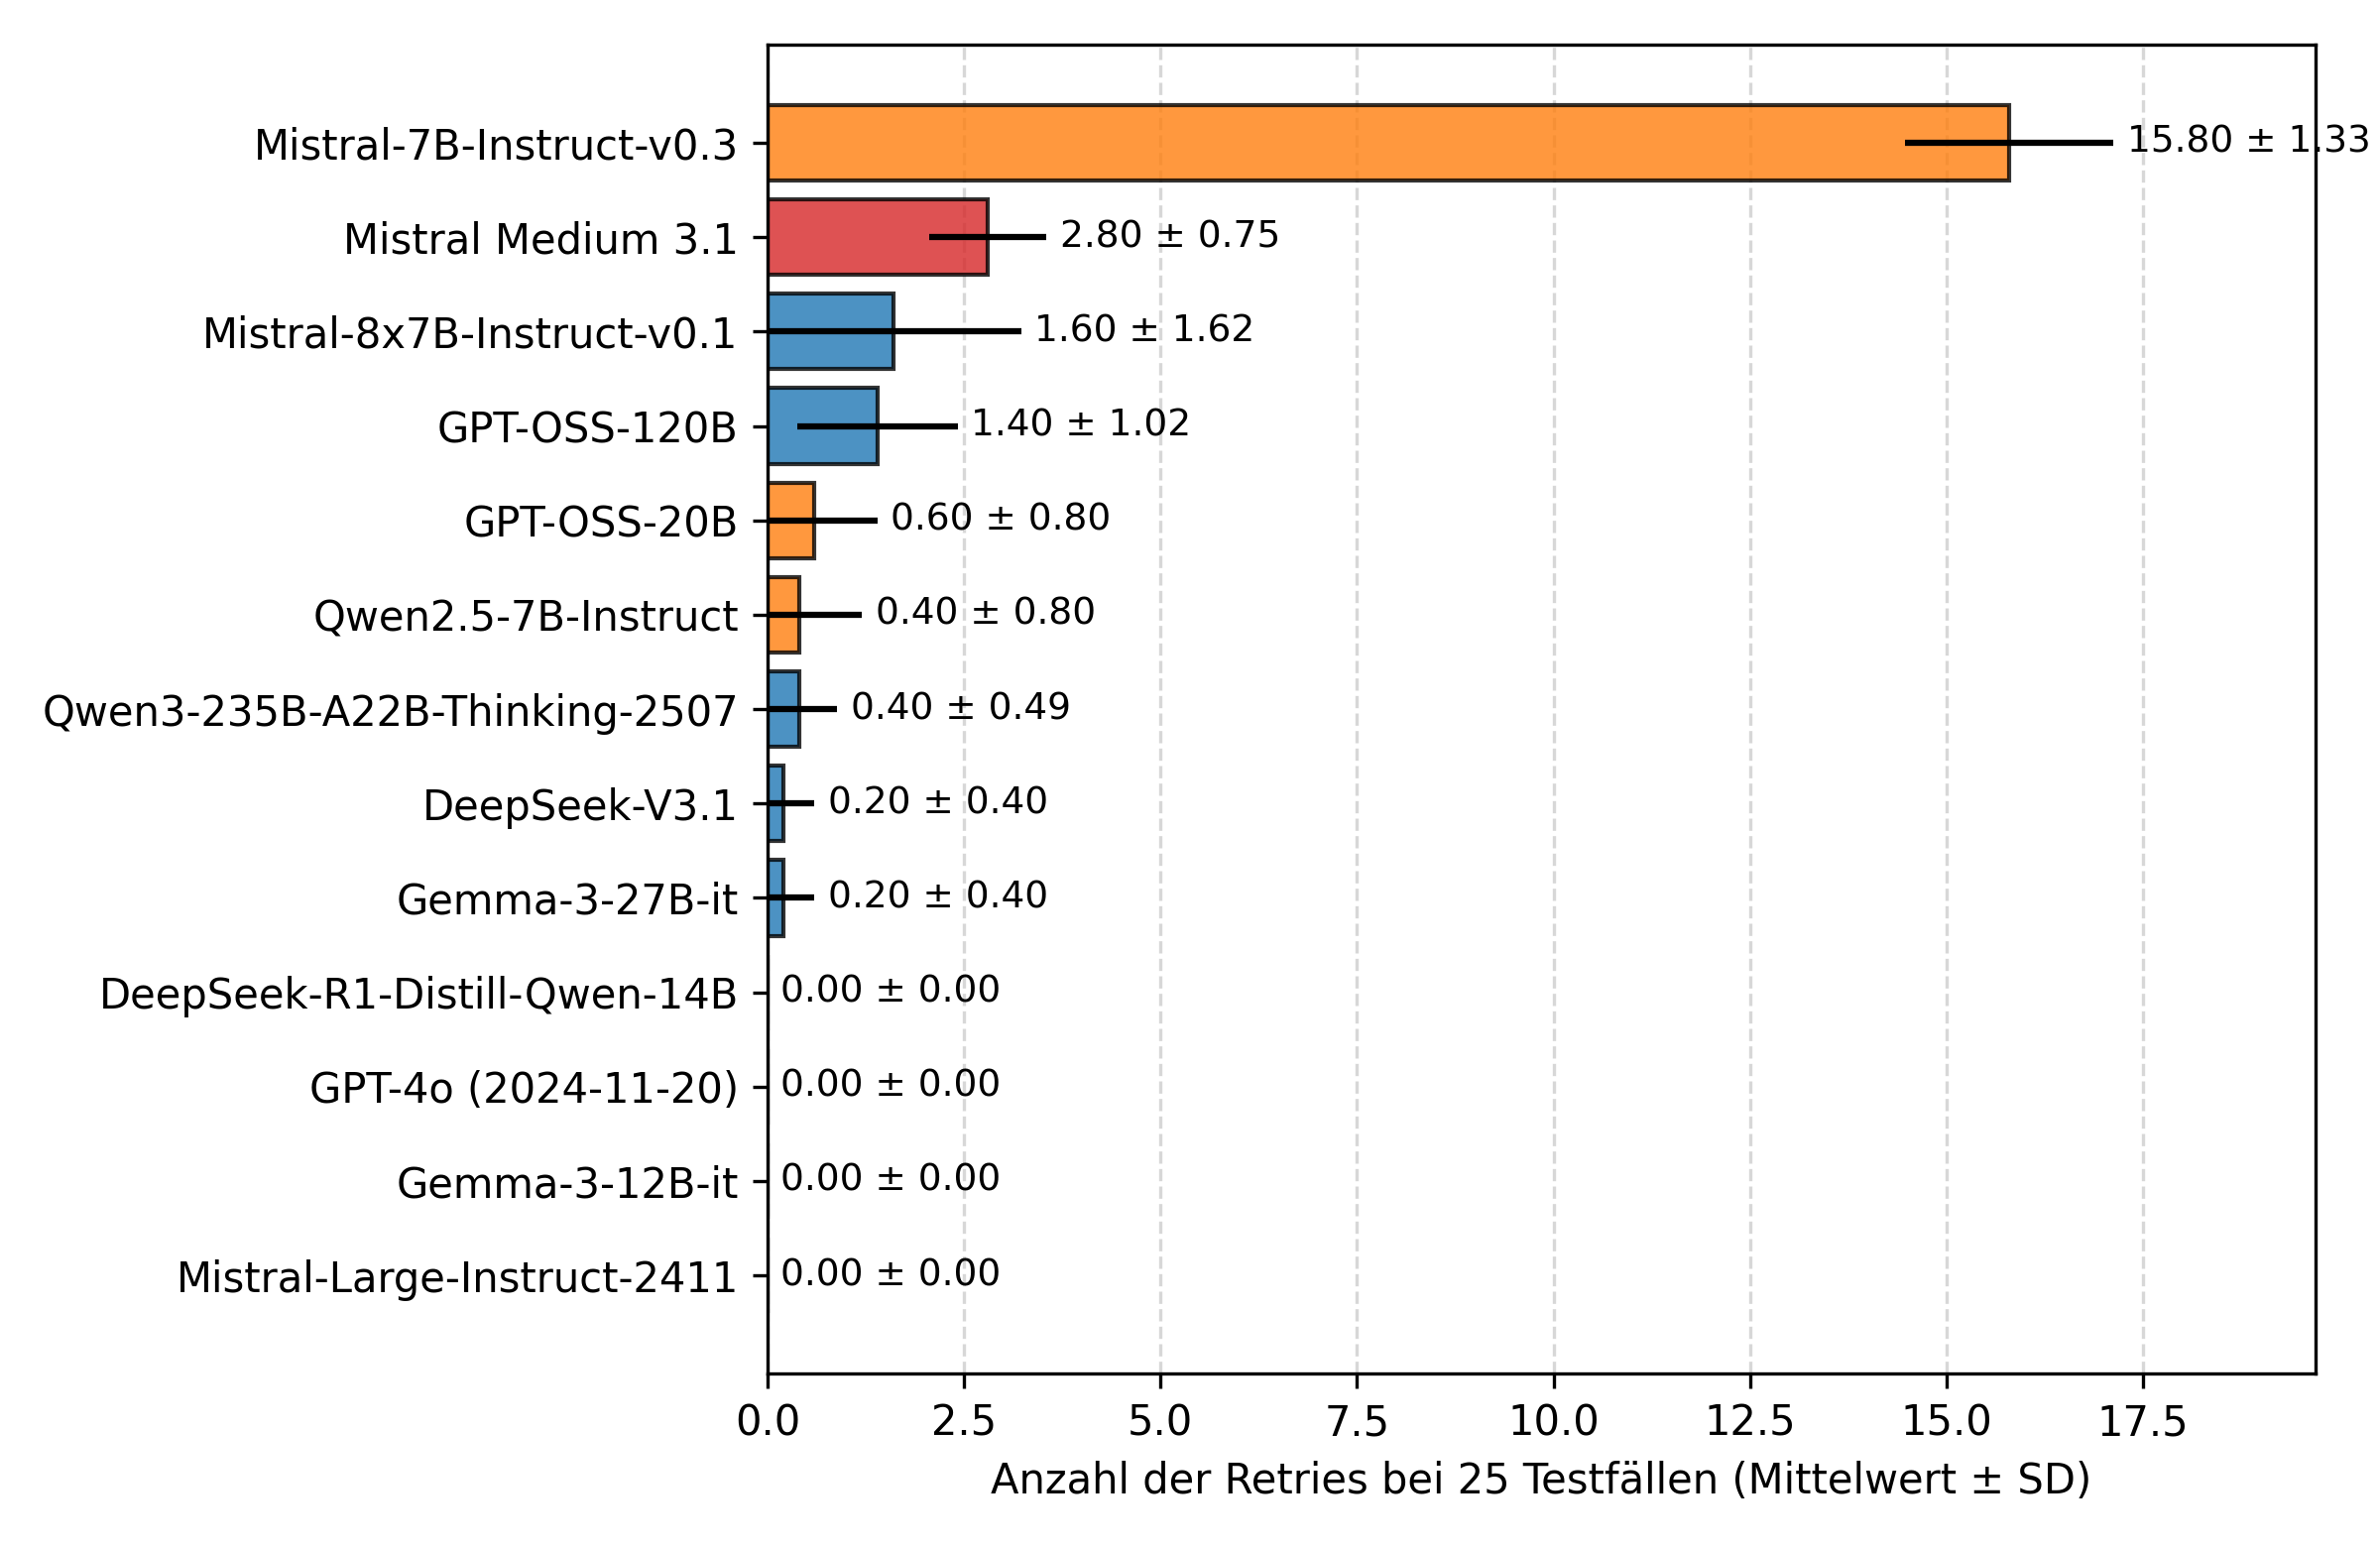
\includegraphics[width=0.9\textwidth]{images/results/evaluation_amount_of_retries}
    \caption{Durchschnittliche Anzahl der Retries, die notwendig waren, um für alle 25 Testfälle eine formatkorrekte JSON-Antwort zu erhalten.}
    \label{fig:results_evaluation_amount_of_retries}
\end{figure}

Robuste Modelle sollten sowohl in der Varianz der Metriken als auch in der konsistenten korrektheit des Ausgabeformats überzeugen. Die Ergebnisse zeigen, dass offene Modelle wie \texttt{Gemma-3-12B-it}, \texttt{Mistral-Large-Instruct-2411} und\linebreak\texttt{DeepSeek-R1-Distill-Qwen-14B} diese Anforderungen erfüllen: Sie besitzen geringe Standardabweichungen und benötigen keine oder nur sehr wenige Retries. Dagegen schränken eine hohe Varianz der F1‑Scores oder viele erforderliche Wiederholungen, wie es bei \texttt{Mixtral‑8x7B‑Instruct‑v0.1} bzw. \texttt{Mistral-7B-\linebreak~Instruct-v0.3} der Fall ist, die Praxistauglichkeit eines Modells deutlich ein. Im nächsten Abschnitt werden anhand von Fallstudien weitere qualitative Einblicke in die Stärken und Schwächen der Modelle gewonnen.